%% This is an example first chapter.  You should put chapter/appendix that you
%% write into a separate file, and add a line \include{yourfilename} to
%% main.tex, where `yourfilename.tex' is the name of the chapter/appendix file.
%% You can process specific files by typing their names in at the 
%% \files=
%% prompt when you run the file main.tex through LaTeX.
\chapter{Execution Profile of Linux Services} \label{ch:boot}
This chapter provides some background on the
Linux startup process (Section \ref{linuxboot}).  
It then describes how we collected user-level instruction
streams from some Linux services via dynamic instrumentation to 
measure nondeterminism in the Linux boot process (Section \ref{datacollection}).
Finally, it summarizes our results on the statistical nature
of nondeterminism in Linux services (Section \ref{bootresults}).

\section{The Linux Boot Process}\label{linuxboot}
When a computer boots up:
\begin{enumerate}
\item The BIOS (Basic Input/Output System) 
gets control and performs startup tasks for the specific hardware platform.
\item Next, the BIOS reads and executes code from a designated boot device 
that contains part of a Linux boot loader. Typically,
this smaller part (or phase 1) 
loads the bulk of the boot loader code (phase 2).
\item The boot loader may present the user with options for 
which operating system to load (if there are multiple available options).
In any case, the boot loader loads and decompresses the operating system
into memory; it sets up system hardware and
memory paging; finally, it transfers control to the kernel's
\texttt{start\_kernel()} function.
\item The \texttt{start\_kernel()} function performs the 
majority of system setup (including interrupts, remaining memory
 management, device initialization)
before spawning the \texttt{idle} process, the scheduler
and the user-space \texttt{init} process.
\item The scheduler effectively takes control of system management,
and kernel stays idle from now on unless externally called.
\item The \texttt{init} process executes scripts that set up all
non-operating system services and structures in order to allow 
a user environment to be created, and then presents the user with a login screen.
\end{enumerate}

\begin{figure}[h]
  \centering
  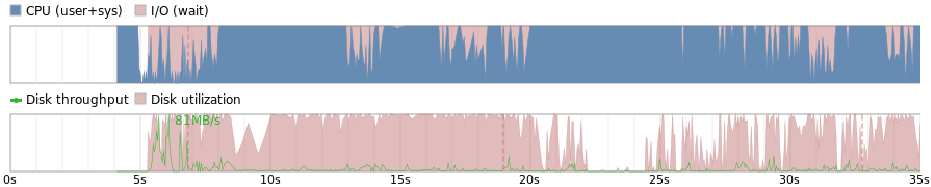
\includegraphics[scale=0.64, trim=1cm 0cm 1cm 0cm]{boot_first35seconds.png}
  \caption[CPU and disk activity for a booting Ubuntu VM in the first 35
  seconds after \texttt{init} is spawned]%
  {CPU and disk activity for a booting Ubuntu VM in the first 35 seconds after \texttt{init} is spawned.
  The first few seconds show no activity because
  the data collection daemon takes a few seconds to start.}
  \label{boot:first35}
\end{figure}

\begin{figure}[h]
  \center
  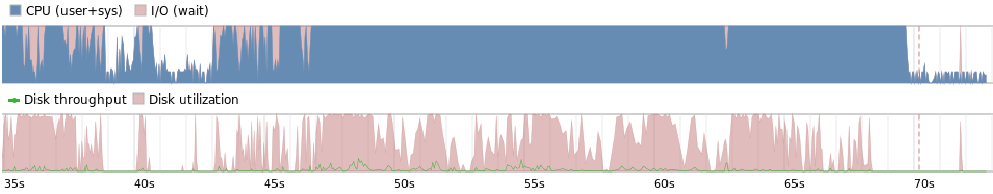
\includegraphics[scale=0.6, trim=1cm 0cm 1cm 0cm]{boot_last35seconds.png}
  \caption[(... continued) CPU and disk activity for a booting VM
  35 seconds after \texttt{init} is spawned. ]%
  {(... continued from Figure \ref{boot:first35}) CPU and disk activity for a booting Ubuntu VM 35 seconds after \texttt{init} is spawned.}
  \label{boot:last35}
\end{figure}

Figures \ref{boot:first35} and \ref{boot:last35}
illustrate the CPU usage and disk activity 
of an Ubuntu 10.10 VM that takes about 70 seconds
to complete the sixth step of the boot process (i.e. spawning 
the \texttt{init} process to set up the user environment).
The Linux kernel version is 2.6.35-27-generic
and the VM is configured with a single core processor
with 512 MB RAM. Generated using
the Bootchart utility \cite{mahkovec2005bootchart},
the figures illustrate that
the booting process involves high memory
and CPU overhead (5-70 seconds); they also 
show a glimpse of the well-known fact that memory and CPU
overhead typically dimishes greatly after the boot
process is completed and the machine is
ready for login (70+ seconds). This disparity
in CPU/memory usage is the source of the boot storm problem;
a single host can handle many VMs in
steady-state usage but gets crippled
when the same VMs boot up concurrently.

In the last step of the booting
process (step 6), \texttt{init} typically
runs many scripts located in 
specific directories such as \texttt{`/etc/rc'}
or \texttt{`/etc/init.d/'}. While the myriad Linux distributions
can have their own variants of \texttt{init} binaries
(e.g. \texttt{SysV}, or \texttt{systemd} or \texttt{Upstart}),
the \texttt{init} process always directly/indirectly launches several 
services and daemons to initialize the user desktop
environment. Figure \ref{boot:services} provides a
summary of the specific actions performed by \texttt{init} 
(through the subprocesses or daemons it launches)
for the same Ubuntu VM used for 
Figures \ref{boot:first35} and \ref{boot:last35}.

\begin{figure}[h]
  \center
  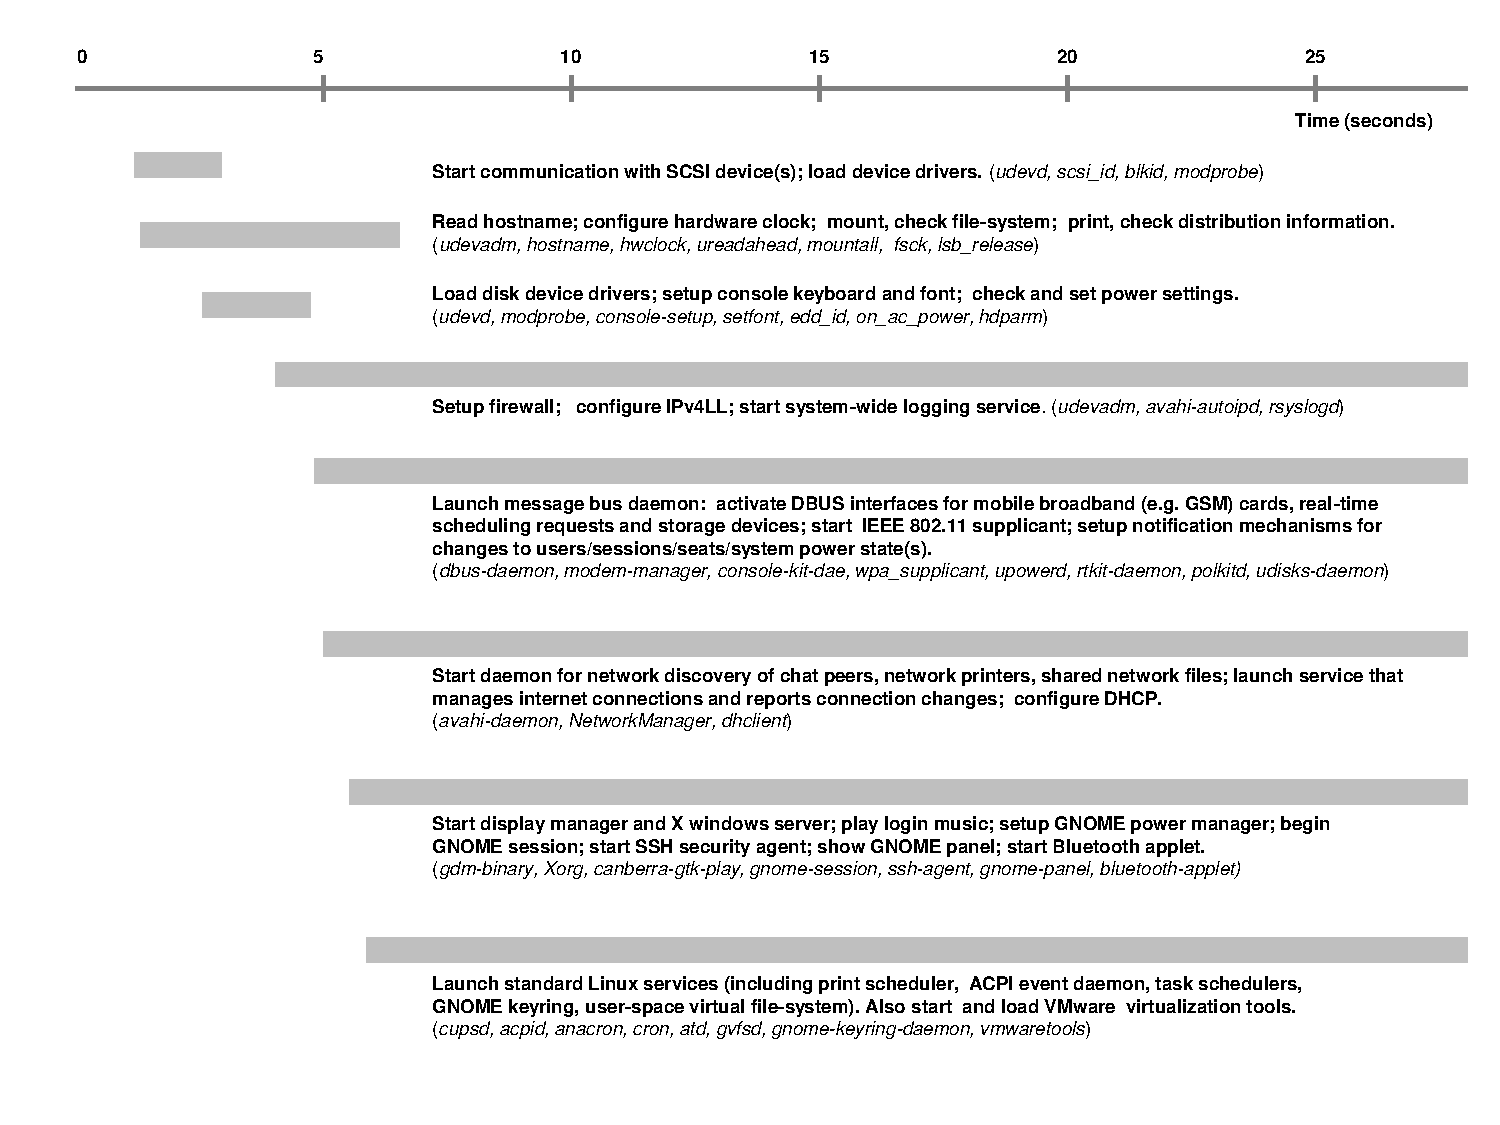
\includegraphics[width=1.0\textwidth, trim=0.5cm 1cm 1cm 1cm]{boottimeline.pdf}
  \caption[A summary of the actions performed by \texttt{init} for a booting VM]%
  {A summary of the actions performed by \texttt{init} for a booting VM;
  this figure has the same timeline (0-70 seconds) as Figures \ref{boot:first35} and 
  \ref{boot:last35}.}
  \label{boot:services}
\end{figure}

In fact, the \texttt{init} process actually launched 361 children processes (directly
and indirectly) over the 70 second period summarized by Figure \ref{boot:services}.
Most of them were ephemeral processes; several processes were repeatedly launched
in different contexts (e.g. \texttt{getty} or \texttt{grep}). The processes singled out
in Figure \ref{boot:services} are the ones that either 
stayed alive through most of the boot process till the end, performed important
boot actions, or spawned many sub-processes themselves.

\section{Data Collection Scheme} \label{datacollection}
\begin{figure}[h]
  \center
  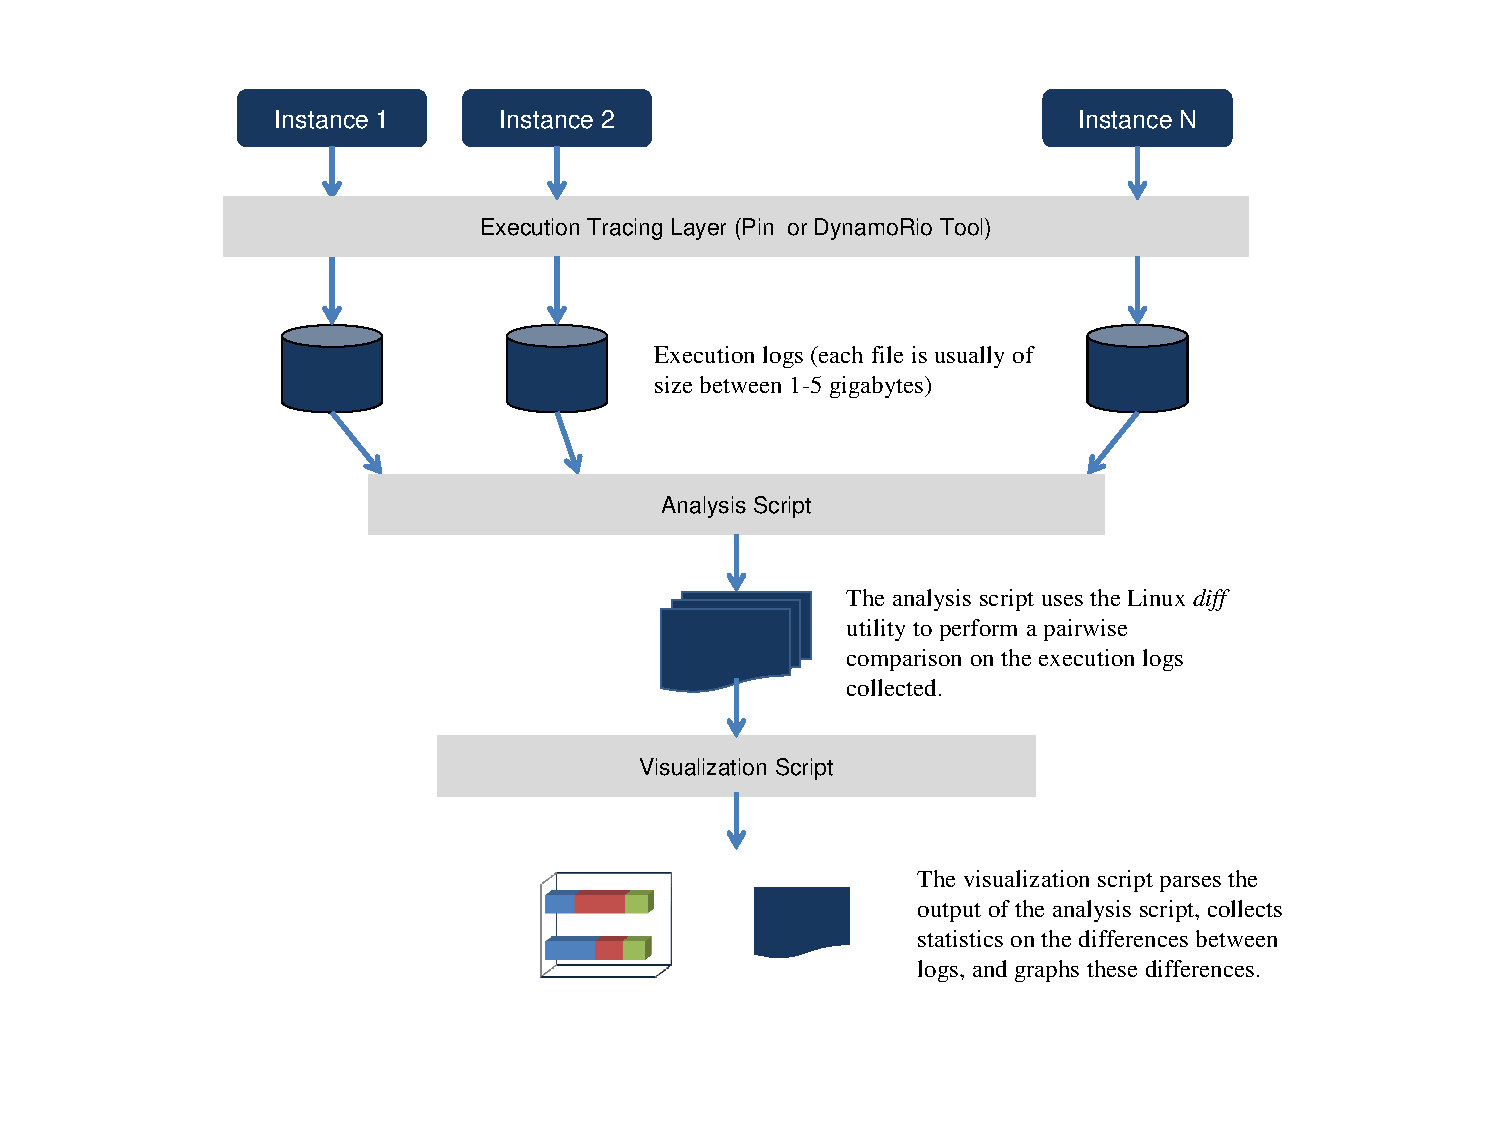
\includegraphics[width=1.0\textwidth, trim=1cm 1cm 1cm 1cm]
                  {naivedatacollection.pdf}
  \caption[Steps involved in measuring execution nondeterminism]%
  {Steps involved in measuring execution nondeterminism.}
  \label{data:naive}
\end{figure}

Pin and DynamoRio are runtime frameworks that enable inspection
and arbitrary transformation of user-mode application code as it executes.
We used both Pin and DynamoRio to study the behavior
of Linux services in order to verify
the accuracy of our results. However, we relied on Pin more 
than DynamoRio because it gets injected into application code
earlier than DynamoRio and thus provides greater
instruction coverage for our purpose.  Figure \ref{data:naive} shows the simple steps involved
in collecting data on nondeterminism using
dynamic instrumentation. The next section 
explains each of these steps in detail, 
using a simple ``Hello, world!'' program as an example.

\subsection{Measuring nondeterminism in a simple $C$ program} \label{ch:hw}
This section outlines the data collection scheme
described in Figure \ref{data:naive} in detail with the help
of an example:  the simple ``Hello, world!'' program
outlined in Figure \ref{source:hw}.
For this example, we disabled ASLR (Address Space Layout
Randomization) on the Ubuntu VM described in section \ref{linuxboot}. \newline

\begin{figure}[h]
  \lstset{frame=shadowbox, rulesepcolor=\color{Gray},
    basicstyle=\small, numbers=left, numberstyle=\footnotesize}
  \lstinputlisting[language=C]{helloworld.c}
  \caption[A ``Hello, world!'' program in C.]%
          {A ``Hello, world!'' program in C. }
          \label{source:hw}
\end{figure}

\noindent {\bf Execution Tracing Layer} \newline
As shown in Figure \ref{data:naive}, the first step
in data collection involves running the target program
a few times across identical VMs. Ideally, these 
different executions are done concurrently or as
close as possible in time to model the boot storm scenario accurately. 
In our scheme, we wrote a Pin tool that:
\begin{enumerate}
\item logs each x86 instruction executed by 
  the target process, along with the 
  new values of any affected registers, 
\item records values written to or 
  read from memory,
\item intercepts all signals received, and records the instruction counts 
  corresponding to the timing of any signals, and
\item monitors all system calls made by the target process,
  and logs any corresponding side-effects to memory or registers.
\end{enumerate}

At present, our Pin tool traces the main process 
for an application and 
does not follow any child processes 
spawned by it for simplicity. This prevents
us from including the user-mode
instructions executed from child processes in our traces, but we get 
sufficiently high coverage to get a good understanding 
of the target program's behavior. We 
treat spawned child processes as part of the outside
world, and trace their interactions with the original process
(e.g. via signals or pipes).

Implementation of the execution tracing layer required
a close examination of the Linux system call interface,
because we had to identify the side-effects of each system call. 
Figure \ref{hw:logsys} shows an excerpt from a trace 
generated by our Pin tool while running the ``Hello, World'' 
program. Our tool records 
every instruction executed in user-space by the process
for the ``Hello, world'' program once Pin gets control; 
this allows us to include program initialization
and library code in our analysis. \newline

\begin{figure}[h]
  \center
  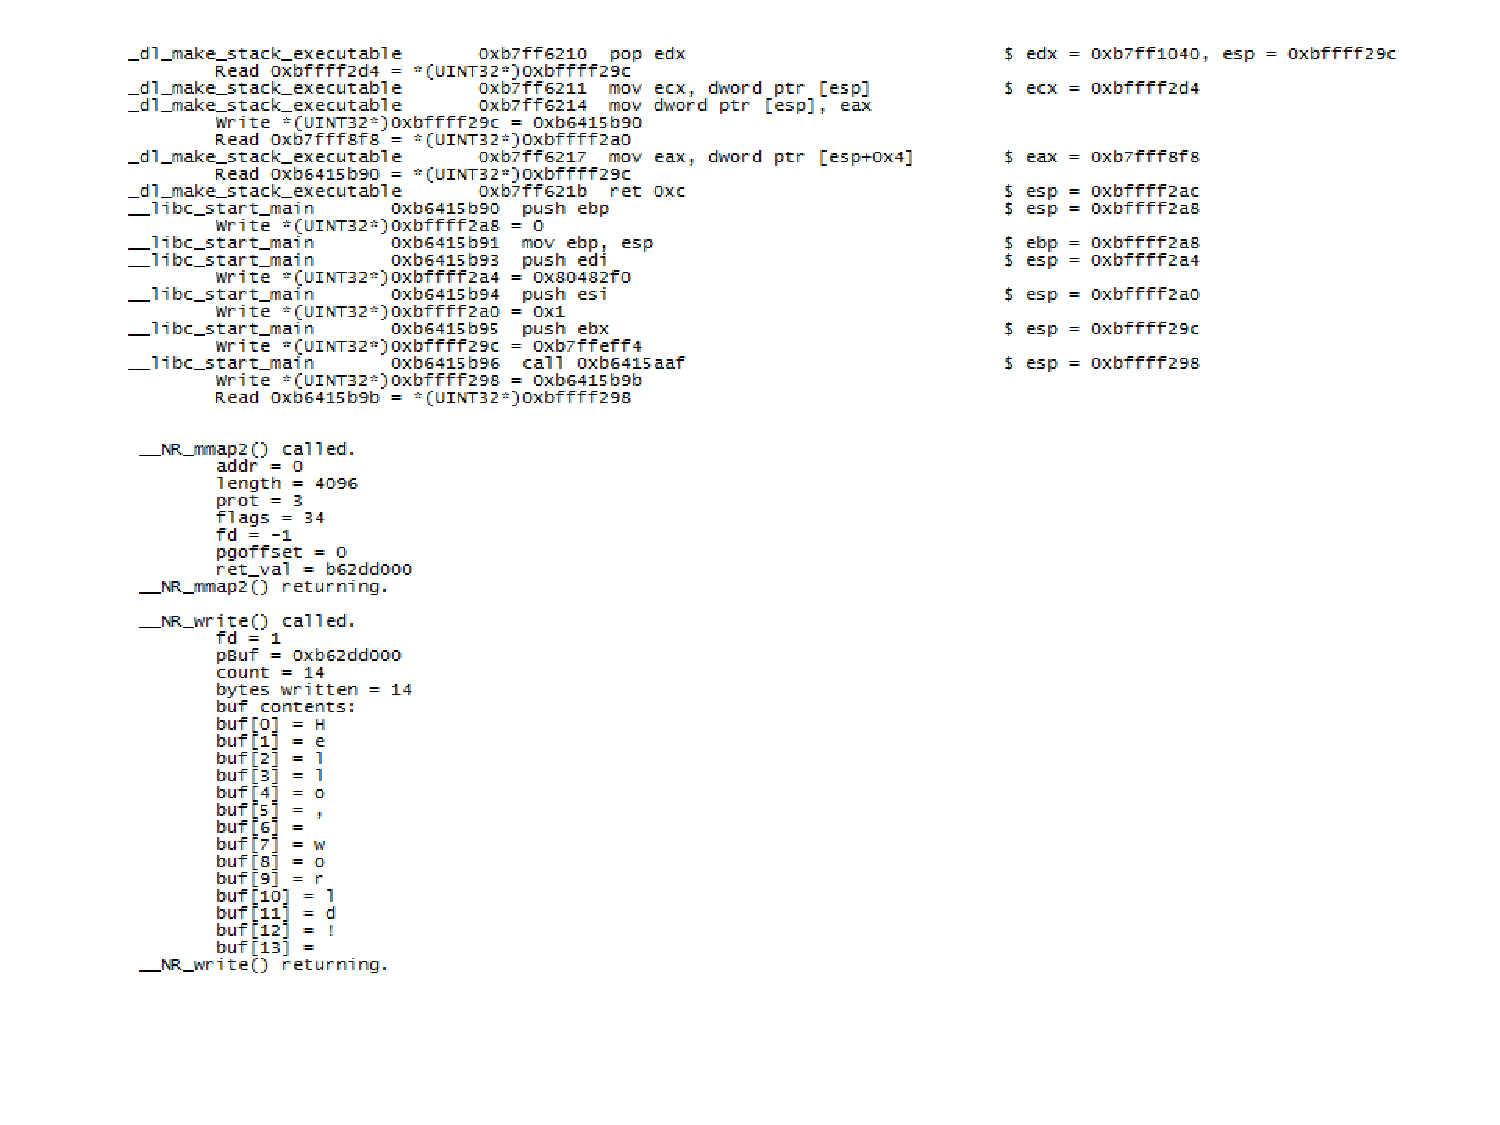
\includegraphics[scale=0.50, trim=2cm 2cm 2cm 0.5cm]{log.pdf}
  \caption[Excerpts from the log files generated by the execution tracing layer]%
          {Excerpts from the log files generated by the execution tracing layer.
          The top half shows x86 instructions executed 
          in user-space by the ``Hello, world!'' process, including instruction addresses, 
          limited symbolic information, affected register values and memory 
          addresses. The lower half shows part of the system call log.}
  \label{hw:logsys}
\end{figure}

\noindent {\bf Analysis Script} \newline
The analysis script uses the Linux \emph{diff} utility
to perform pairwise comparisons of the log files generated 
by multiple executions of the target application. 
Using the \texttt{suppress-common}, \texttt{side-by-side}
and \texttt{minimal} flags, the analysis script
produces two output files: 
\begin{enumerate}
\item A {\em delta} file
that contains only instructions that were 
either conflicting between the two logs or missing in one log, and
\item A {\em union} file that contains all instructions
executed in the two logs, while distinguishing instructions  
included in the delta file from others.
\end{enumerate}

\begin{figure}[h]
  \center
  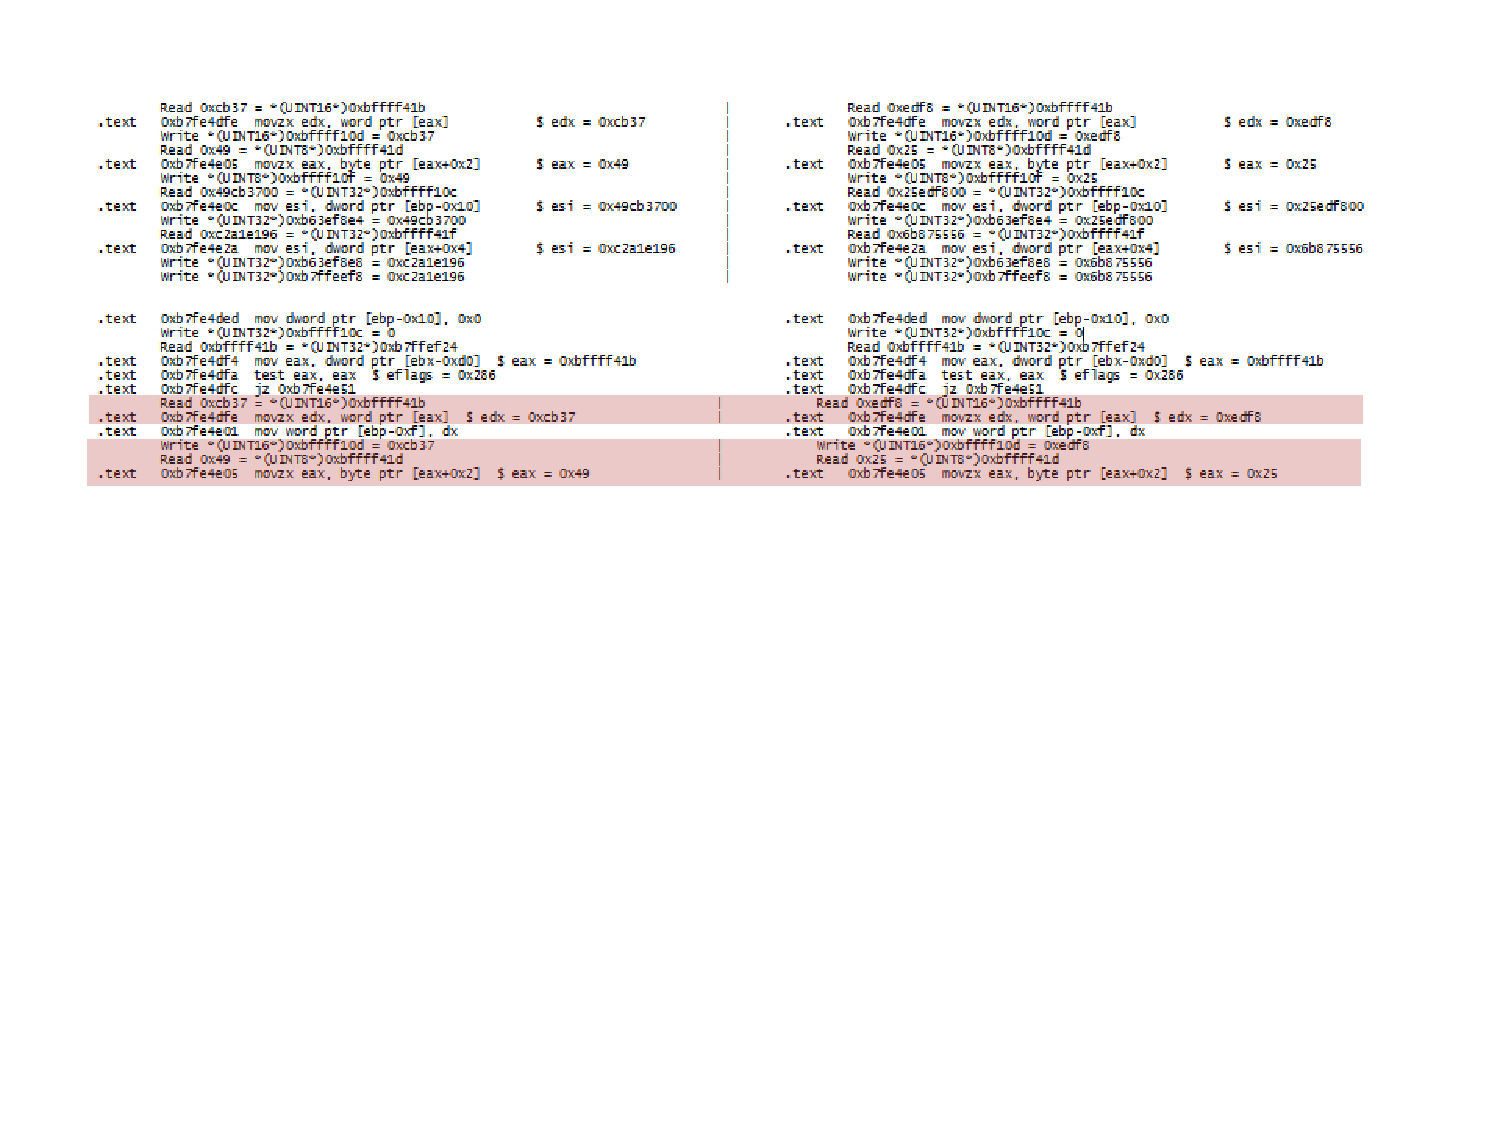
\includegraphics[scale=0.50, trim=3cm 1.5cm 3cm 1.5cm]{log2.pdf}
  \caption[Excerpts from the side-by-side diff files generated by the analysis script]%
          {Excerpts from the diff files generated by the analysis script.
            The top half shows instructions from the delta file;
            these all have different side-effects in the two logs
            (as indicated by the $\vert$).
            The bottom half shows instructions from the union file.
            Conflicting instructions are highlighted; others are found in both logs.}
  \label{hw:logsys2}
\end{figure}

\noindent Figure \ref{hw:logsys2} shows an excerpt from the 
union and delta files generated for the ``Hello, world!''
program. Given several traces, the delta and union
files can be constructed from the two
executions that are the most different 
or have the median difference. The 
much smaller size of the delta file
makes it suitable for diagnosing
sources of nondeterminism
in an application. 
\newpage

\noindent {\bf Visualization Script} \newline
The visualization script reads the union file to 
compute statistics on the extent of any differences in the
original logs, and generates diagrams to 
capture the different execution traces of the program.
 
In particular, it derives three key metrics
after processing the union file:
\begin{enumerate}
\item {\em Length of Common Prefix {\bf (P):}} This is 
the number of instructions common
to both logs starting from the beginning
and up to the point of first divergence.
\item {\em Longest Common Substring {\bf (LS):}}
This is the longest sequence of consecutive instructions 
that are common to both logs.
\item {\em Longest Common Subsequence {\bf (LCS):}}
Intuitively, this is the ``overlap'' in the logs;
it is the length of the longest sequence of identical instructions
in both logs. Instructions in the LCS must be in the same order
in both logs, but they are not required to be adjacent.
\end{enumerate}

For instance, if the first instance of a program
executes the instruction sequence $I_1 = [A, B, C, D, E, F]$,
and the second instance of the same program executes 
the instruction sequence $I_2 = [A, B, X, D, E, F, Y]$,
then: the common prefix is $[A, B]$; the longest
common substring is $[D, E, F]$, and the longest
common subsequence is $[A, B, D, E, F]$. 
In general, the longest common subsequence (LCS) of two traces is
arguably the best indicator of the extent of determinism
in two executions of a program.
The other two metrics are important 
for evaluating the feasibility of deduplication of execution as
a solution to the boot storm problem. In general,
we want the common prefix (P) and the longest common substring (LS)
of the two logs to be as large as possible to
ensure that concurrently booting VMs do not need to branch
execution or communicate with each other too quickly (see Chapter
\ref{ch:design}).

For the ``Hello, world!'' program, if ASLR
is enabled, the two logs have very little
overlap ($< 1\%$), and the common
prefix and longest common substring
are on the order of $10$ instructions.
With ASLR disabled, one may 
expect the two traces to look identical (because
of the simplicity of the program), but
there is still some nondeterminism in the 
instruction sequences (see Table \ref{hw:stats}
and Figure \ref{hw:trace}).

\begin{table}
\caption{Nondeterminism profile of ``Hello, world!'' program (ASLR disabled)}
\label{hw:stats}
\begin{center}
\begin{tabular}{||l|c||}\hline
  Common Prefix & 21.49 percent \\\hline
  Longest Common Substring & 67.70 percent \\\hline
  Longest Common Subsequence & 99.98 percent \\\hline
  Conflict Ratio & 0.02 percent \\\hline
  Conflicting Instructions & 32 \\\hline
\end{tabular}
\end{center}
\end{table}

Figure \ref{hw:trace} shows divergences in program execution
over time. This representation allows
us to visually inspect the union file 
and figure out the distribution and nature of conflicting
instructions. For the ``Hello, world!'' program,
we can see that while divergences were 
spread out near the beginning and end of the program,
they were bursty and short-lived (as indicated
by the thin black lines). This is a common trend, 
even for complex programs such as Linux services,
as discussed in Section \ref{bootresults}.


\begin{figure}[h]
  \center
  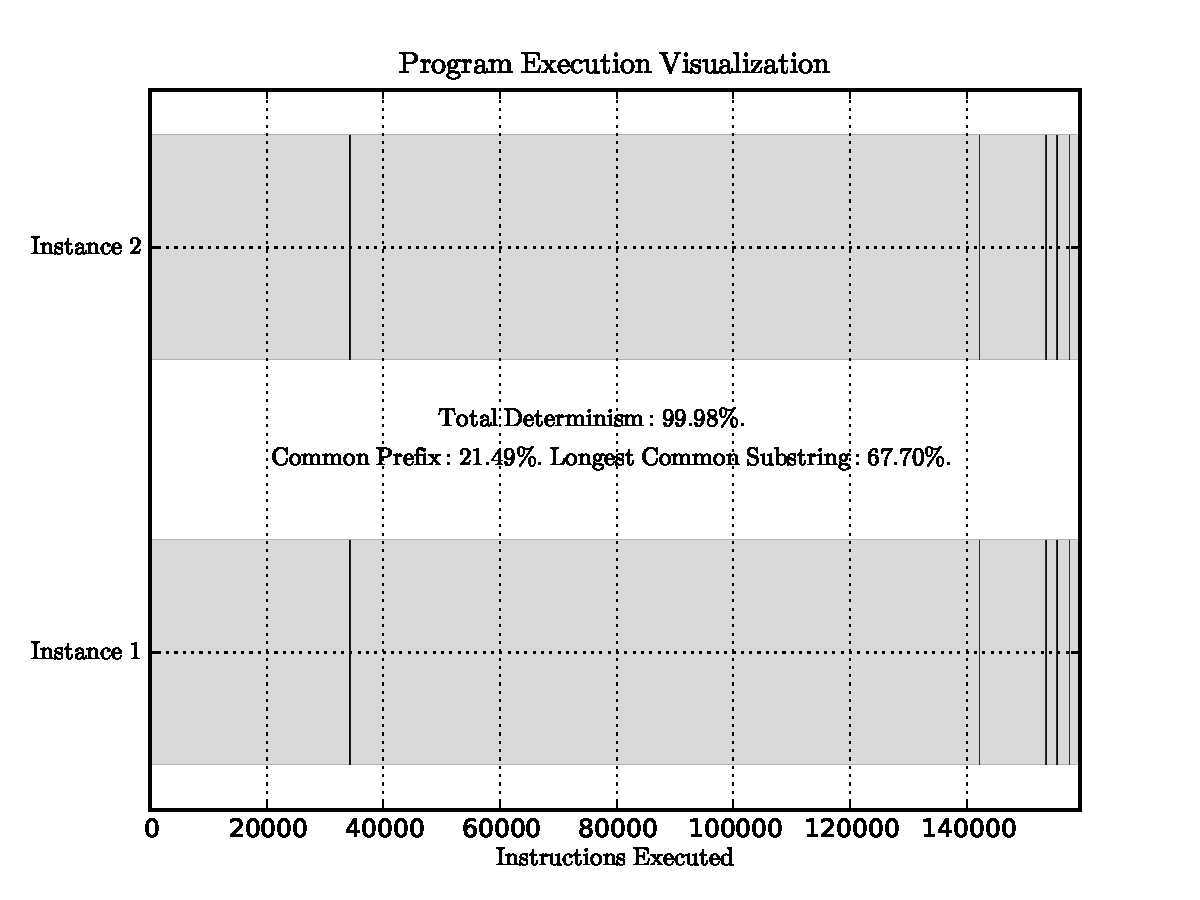
\includegraphics[scale=0.60, trim=0cm 0cm 0cm 0cm]{trace.pdf}
  \caption[Visualization of ``Hello, world!'' program execution]% 
          {Visualization of ``Hello, world!'' program execution.
          The thin black lines represent conflicts between
          the two instances of the program.}
  \label{hw:trace}
\end{figure} 

\subsection{Quantifying Nondeterminism} \label{alt:stats}
As mentioned in the previous section, we use the 
common prefix (P), the longest common subsequence (LCS),
the longest substring (LS) and the distribution of
conflicting instructions in separate instruction
streams to measure nondeterminism.

While the conflict ratio measured by our analysis script is usually quite small (e.g. $0.02\%$
for ``Hello, world!''), its importance and impact is disproportionately larger.
As shown in Figure \ref{cascade:ex},  the analysis script 
ignores the cascade effect and only considers instructions that {\em originate} or actively {\em propagate}
nondeterminism in calculating the conflict ratio. 

\begin{figure}[h]
  \center
  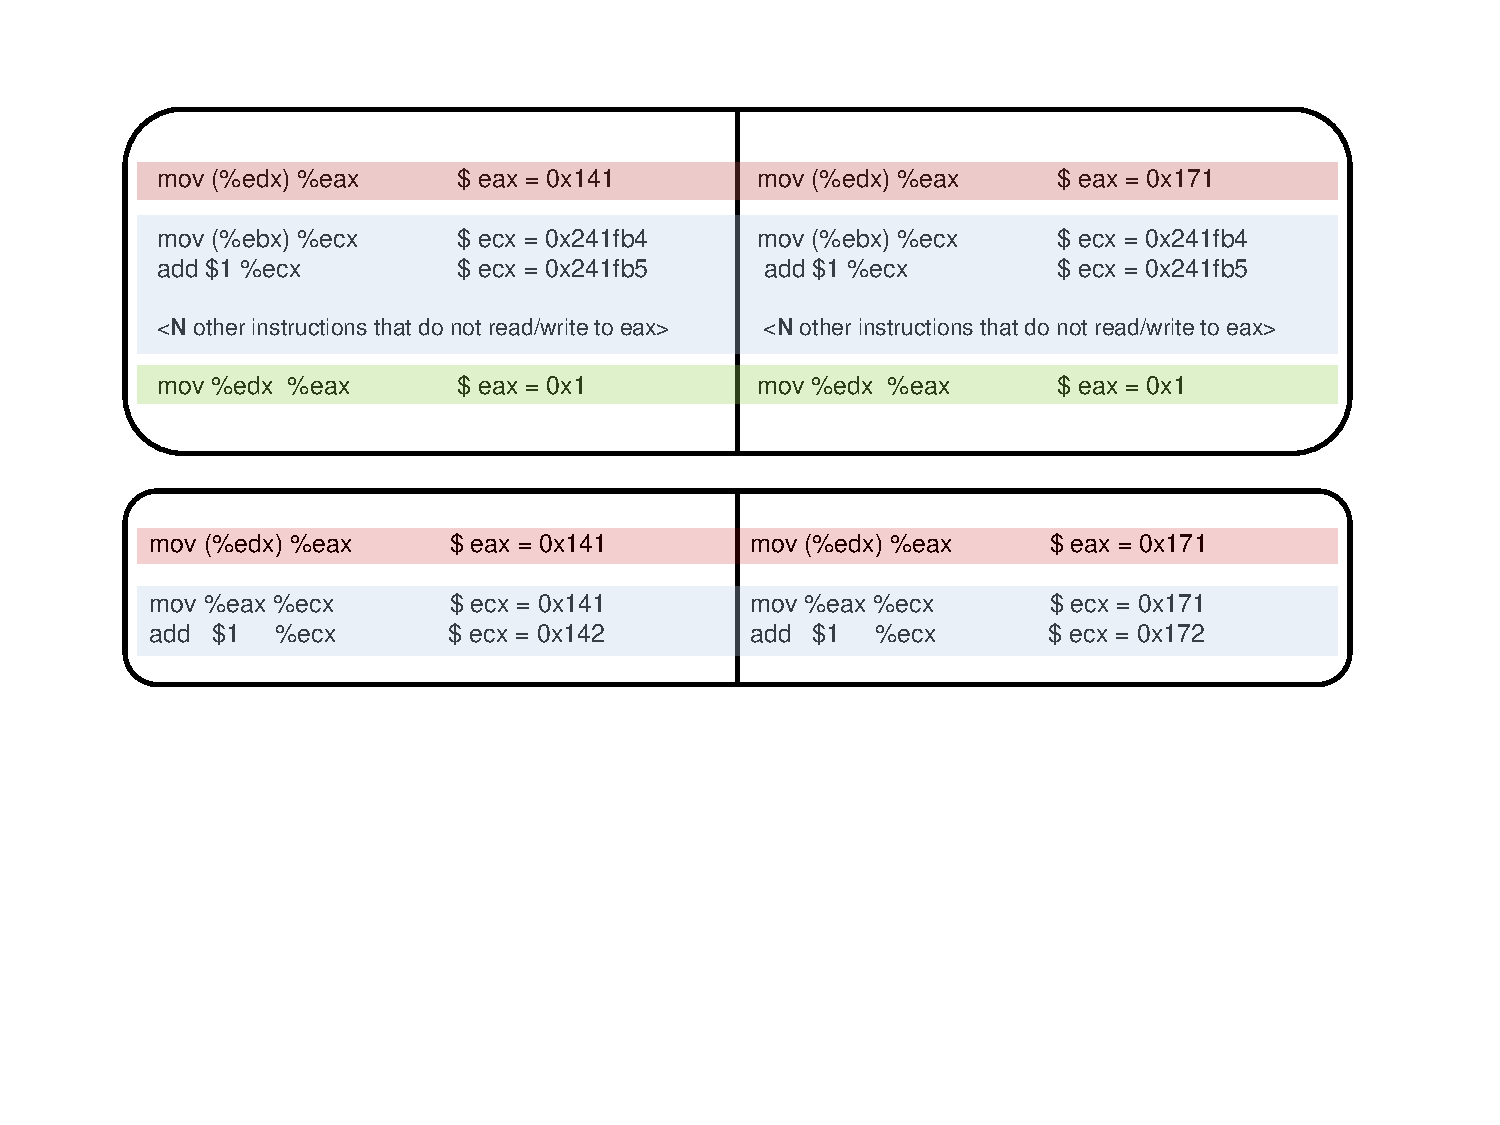
\includegraphics[width=\textwidth, trim=1cm 7cm 1cm 0.4cm]{liveness.pdf}
  \caption[The cascade and propagation effects in measuring nondeterminism.]%
          {The top image shows an example of the cascade effect: the red
          instruction represents a real conflict in \texttt{eax}. The light-blue instructions
          have the same side-effects across the two logs because they do not touch \texttt{eax}.
          The value of \texttt{eax} is different in the blue instructions and converges 
          only after it is written by the green instruction. The cascade effect refers to the 
          nondeterministic register state
          that results in the light-blue instructions because of an earlier conflict, even
          though the instructions themselves are not reading or writing any nondeterministic
          values. If we included the cascade effect, the measured conflict ratio in this
          trace excerpt is $(N+3)/(N+4)$ instead of the $1/(N+4)$ we will report.  \newline
          
          The bottom image shows an example of the propagation effect: the red instruction again
          represents a conflict in \texttt{eax}. The light-blue instructions do not generate
          any nondeterminism themselves, but they have conflicting side-effects because they
          read \texttt{eax}. In this case, we report a conflict ratio of $1$.}
  \label{cascade:ex}
\end{figure} 

\newpage \noindent Since it ignores the cascade effect and 
includes the propagation effect, we effectively simulate a form of {\em taint}
analysis on register and memory contents to measure the
true impact of any nondeterminism in a program. 
Our approach automatically groups instructions that generate and propagate
nondeterminism in the delta files, making it easier for us to 
diagnose the sources of nondeterminism.

One element missing from our study of nondeterminism is that
we do not account for timing-related
nondeterminism directly. For instance, two programs
that execute precisely the same set of instructions but 
take different amounts of time doing so (e.g. due
to variable latency of blocking system calls) are
fully deterministic according to our definition.
We deliberately exclude timing considerations because
it is acceptable for some VMs to lag behind others in the boot storm
scenario, as long as the same instructions are executed.
When timing-related nondeterminism affects program execution
e.g. through differences in signal delivery, I/O ordering
or time-related system calls (see Chapter \ref{ch:src}),
it automatically gets factored in our analysis.

\section{Results for Linux services} \label{bootresults}
Table \ref{hw:stats} shows the results from applying our data
collection scheme on a set of Linux services and daemons
that are typically launched at boot. 

\begin{table}[h]
\caption{Nondeterminism profile of Linux services and daemons (ASLR disabled)}
\label{linux:stats}
\begin{center}
\begin{tabular}{||l|c|c|c||}\hline
  Application & Prefix (P) & Longest Substring (LS) &
  Determinism (LCS) \\
  \hline \hline
  \texttt{ntp}, 14 loop iterations & 11.65\% & 22.08\% & 89.21\%
  \\\hline
  \texttt{cron}, 30 loop iterations & 1.58\% & 53.21\% & 98.38\% 
  \\\hline 
  \texttt{cups}, 10 loop iterations & 2.45\% & 25.20\% & 94.25\%
  \\\hline 
  \texttt{daemon A}, $i$ loop iterations & $p$\% & $ls$\% & $lcs$\%
  \\\hline 
  \texttt{daemon B}, $i$ loop iterations & $p$\% & $ls$\% & $lcs$\%
  \\\hline 
  \texttt{daemon C}, $i$ loop iterations & $p$\% & $ls$\% & $lcs$\%
  \\\hline 
  \texttt{daemon D}, $i$ loop iterations & $p$\% & $ls$\% & $lcs$\%
  \\\hline 
  \texttt{daemon E}, $i$ loop iterations & $p$\% & $ls$\% & $lcs$\%
  \\\hline 
  \texttt{daemon F}, $i$ loop iterations & $p$\% & $ls$\% & $lcs$\%
  \\\hline 
  \texttt{daemon G}, $i$ loop iterations & $p$\% & $ls$\% & $lcs$\%
  \\\hline 
  \hline 
  {\bf Aggregate} & {\bf $x$}\% & {\bf $y$}\% & {\bf $z$}\%
  \\\hline 

\end{tabular}
\end{center}
\end{table}

We can immediately see that:
\begin{enumerate}
\item The common prefix (P) 
in our sample of Linux services is on average about $3\%$,
which is quite small and indicates that nondeterminism 
typically surfaces relatively early in program execution. 

\item The longest substring (LS), usually close to $25\%$,
is substantially larger than the common prefix (P).
This shows that execution typically does not permanently
diverge after the initial differences.

\item The longest common subsequence (LCS) or general determinism
is in general much higher -- about $90\%$ on average -- 
which indicates that a large majority of instructions 
in the Linux services overlap across
different executions. 

\end{enumerate}

Given the discussion in Section \ref{alt:stats}, a conflict ratio
of about $10\%$ on average hints that there is a non-trivial amount of nondeterminism 
in our sample programs, despite a very high average LCS.
The distribution of the $10\%$ conflicting instructions
is surprisingly similar across different programs.

\begin{figure}
  \center
  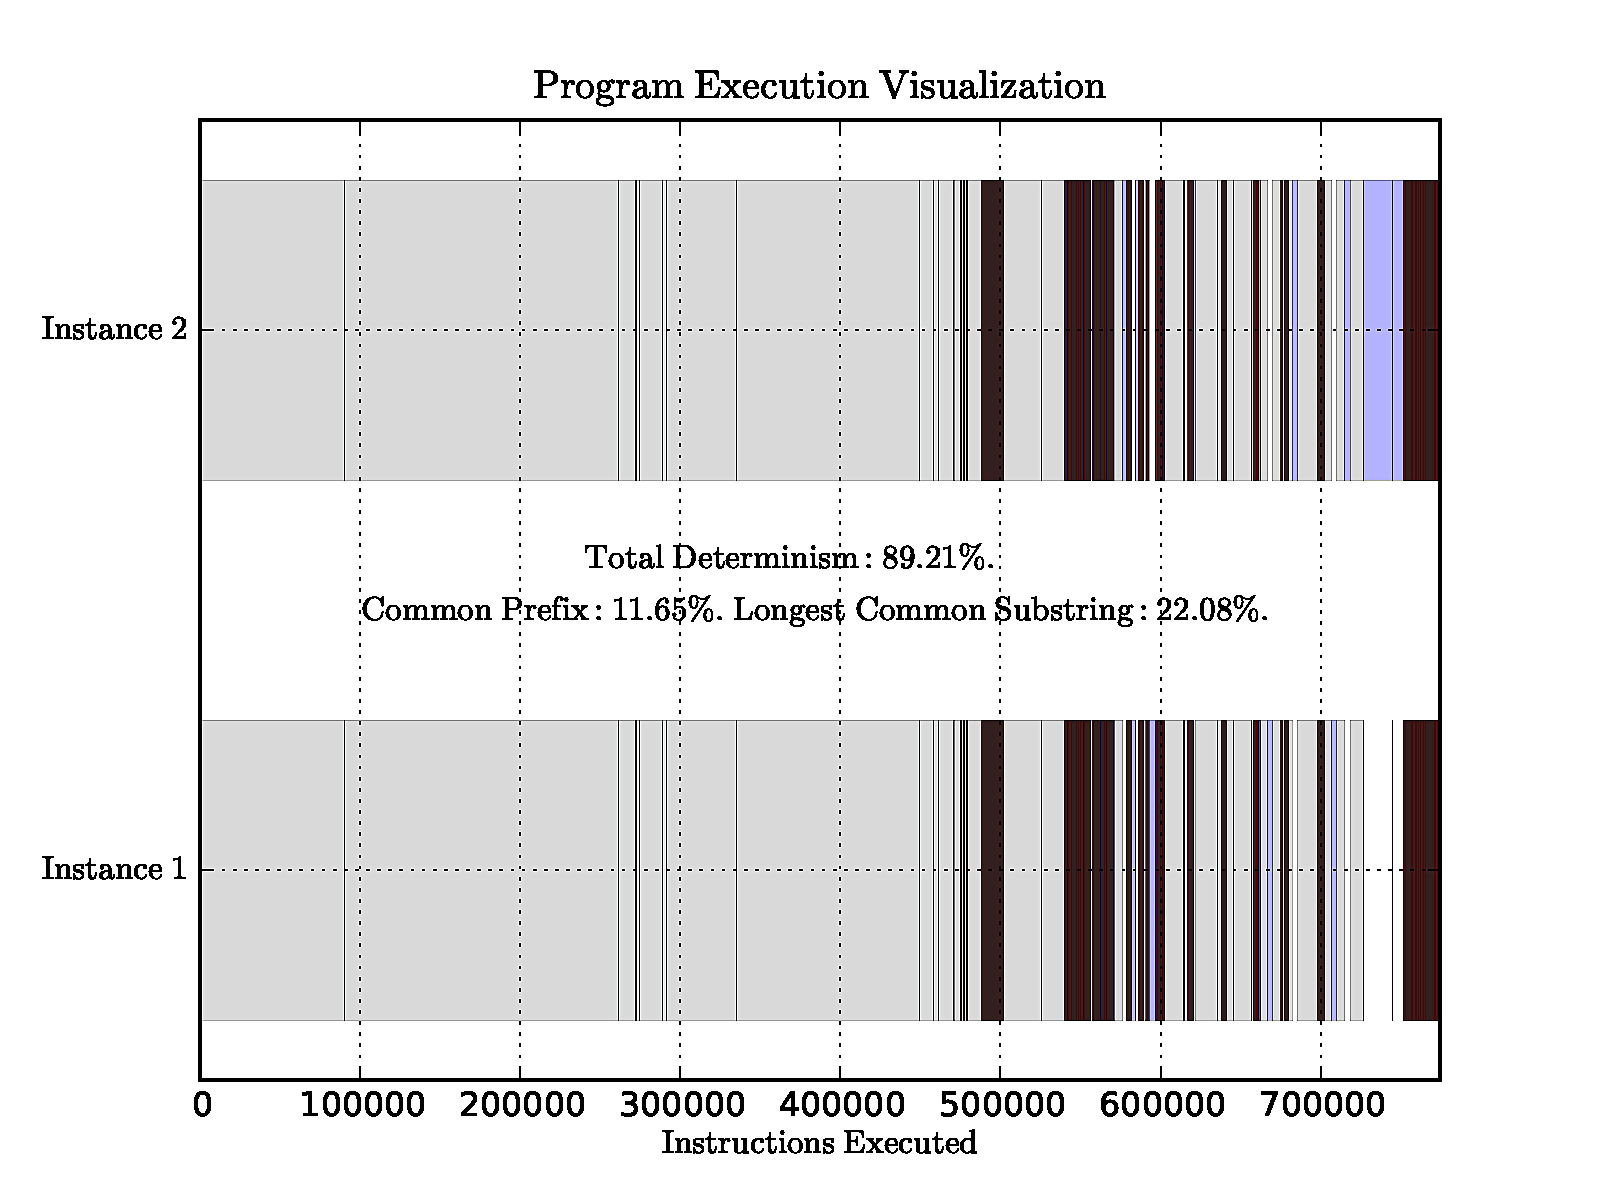
\includegraphics[trim=0cm 0cm 0cm 0cm, width=0.8\textwidth]{ntp-ch2.png}
  \caption[Visualization of \texttt{ntp} program execution]% 
          {Visualization of \texttt{ntp} program execution.
          The thin black lines represent conflicts between
          the two instances of the program, whereas
          the thin blue lines represent control flow
          divergences.}
  \label{ntp:tracech2}
\end{figure} 

Figure \ref{ntp:tracech2}, an execution profile of \texttt{ntp}, is representative
of most execution traces. Generally,
conflicting instructions are spread throughout
the program execution, but tend to occur more frequently
towards the end. Nondeterminism does not seem to cause permanent 
execution divergences, even though there is nontrivial amount
of control-flow divergence in some programs. In fact, execution seems to
diverge and reconverge very frequently.
The execution profile of \texttt{cron} is somewhat unique
because it has a higher LCS and LS than other traces. It is
difficult to reconcile the low measured conflict ratio for \texttt{cron} (less
than $2\%$), with the higher conflict ratio visually suggested by 
Figure \ref{cron:tracech2}. Figure \ref{cron:zoomtracech2} 
explains this discrepancy: it shows that while
the absolute number of conflicting instructions is small,
these conflicts occur in bursts and visually group together. 
While the bursty nature of nondeterminism
is particularly prominent in Figure \ref{cron:zoomtracech2},
it is common to all the services we profiled. Table \ref{burst:stats}
shows that the longest control flow divergence 
or the longest string of consecutive conflicts
is typically very small (i.e. $<<1\%$) 
in our sample programs.

\begin{figure}
  \center
  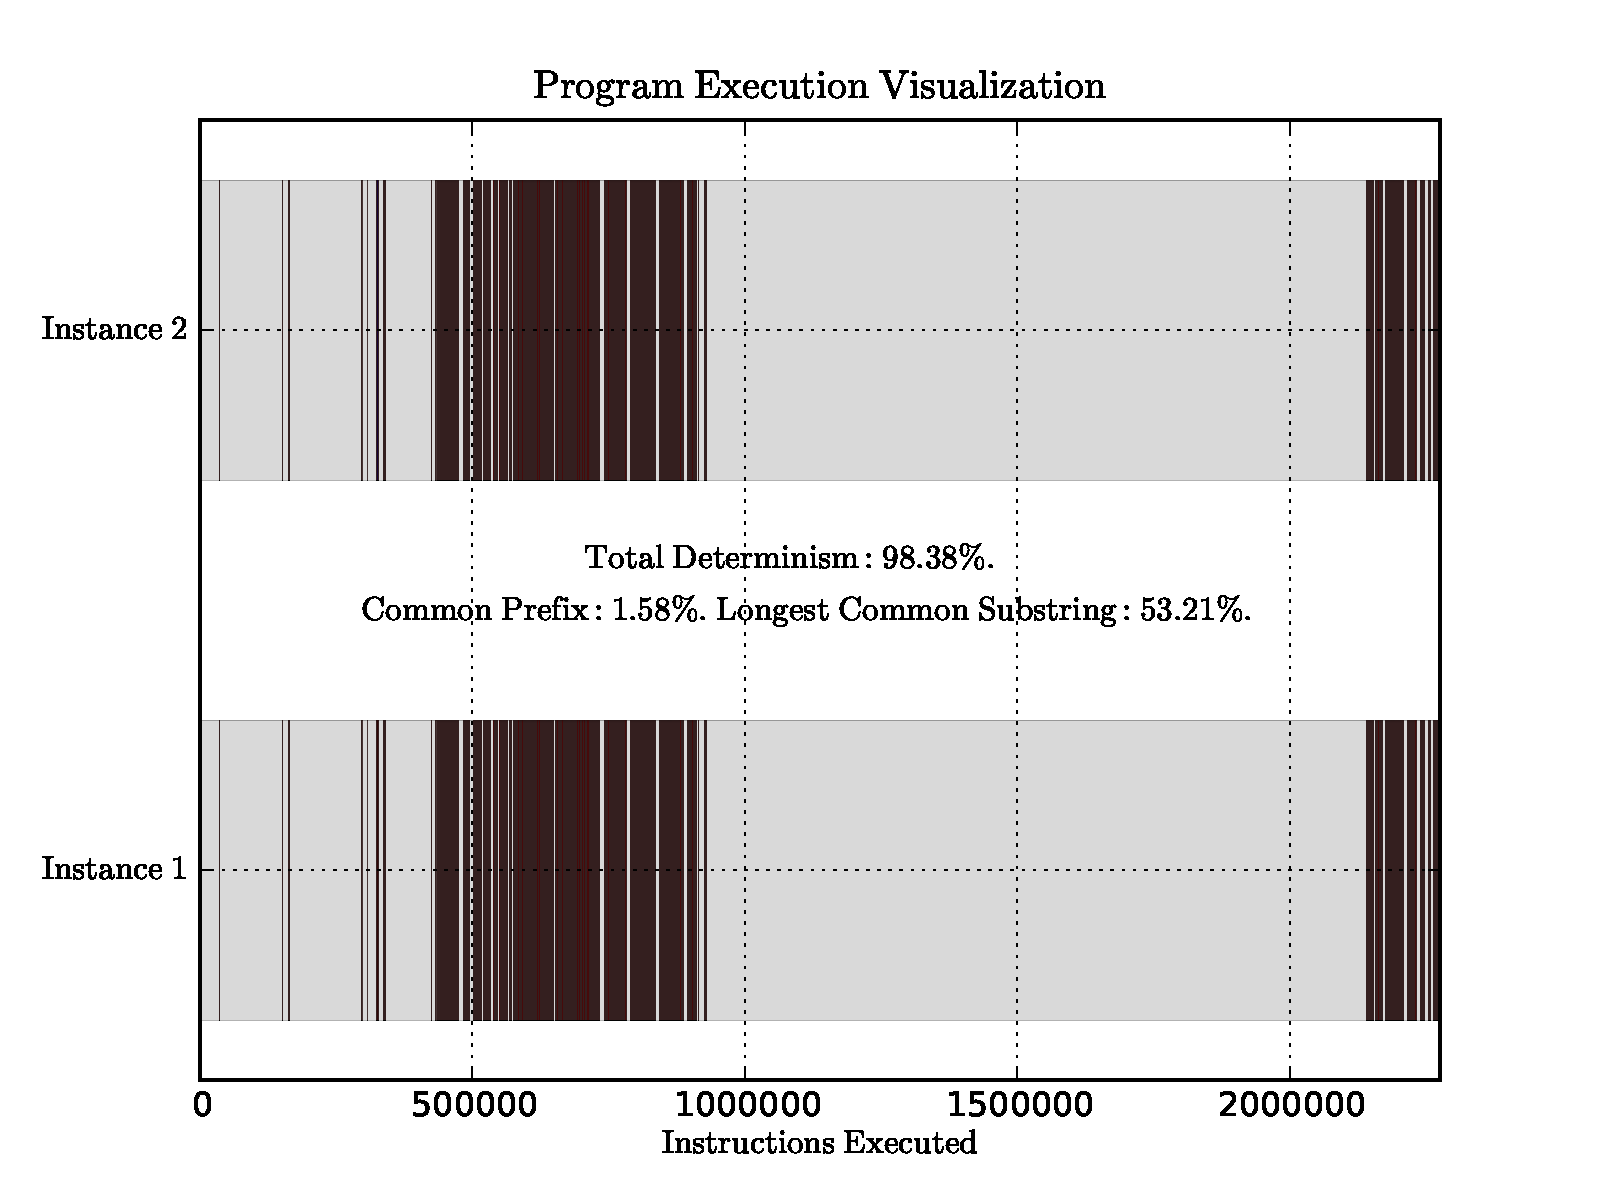
\includegraphics[trim=0cm 0cm 0cm 0cm, width=0.8\textwidth]{cron-ch2.png}
  \caption[Visualization of \texttt{cron} program execution]% 
          {Visualization of \texttt{cron} program execution.
          The thin black lines represent conflicts between
          the two instances of the program.}
  \label{cron:tracech2}
\end{figure} 


\begin{figure}
  \center
  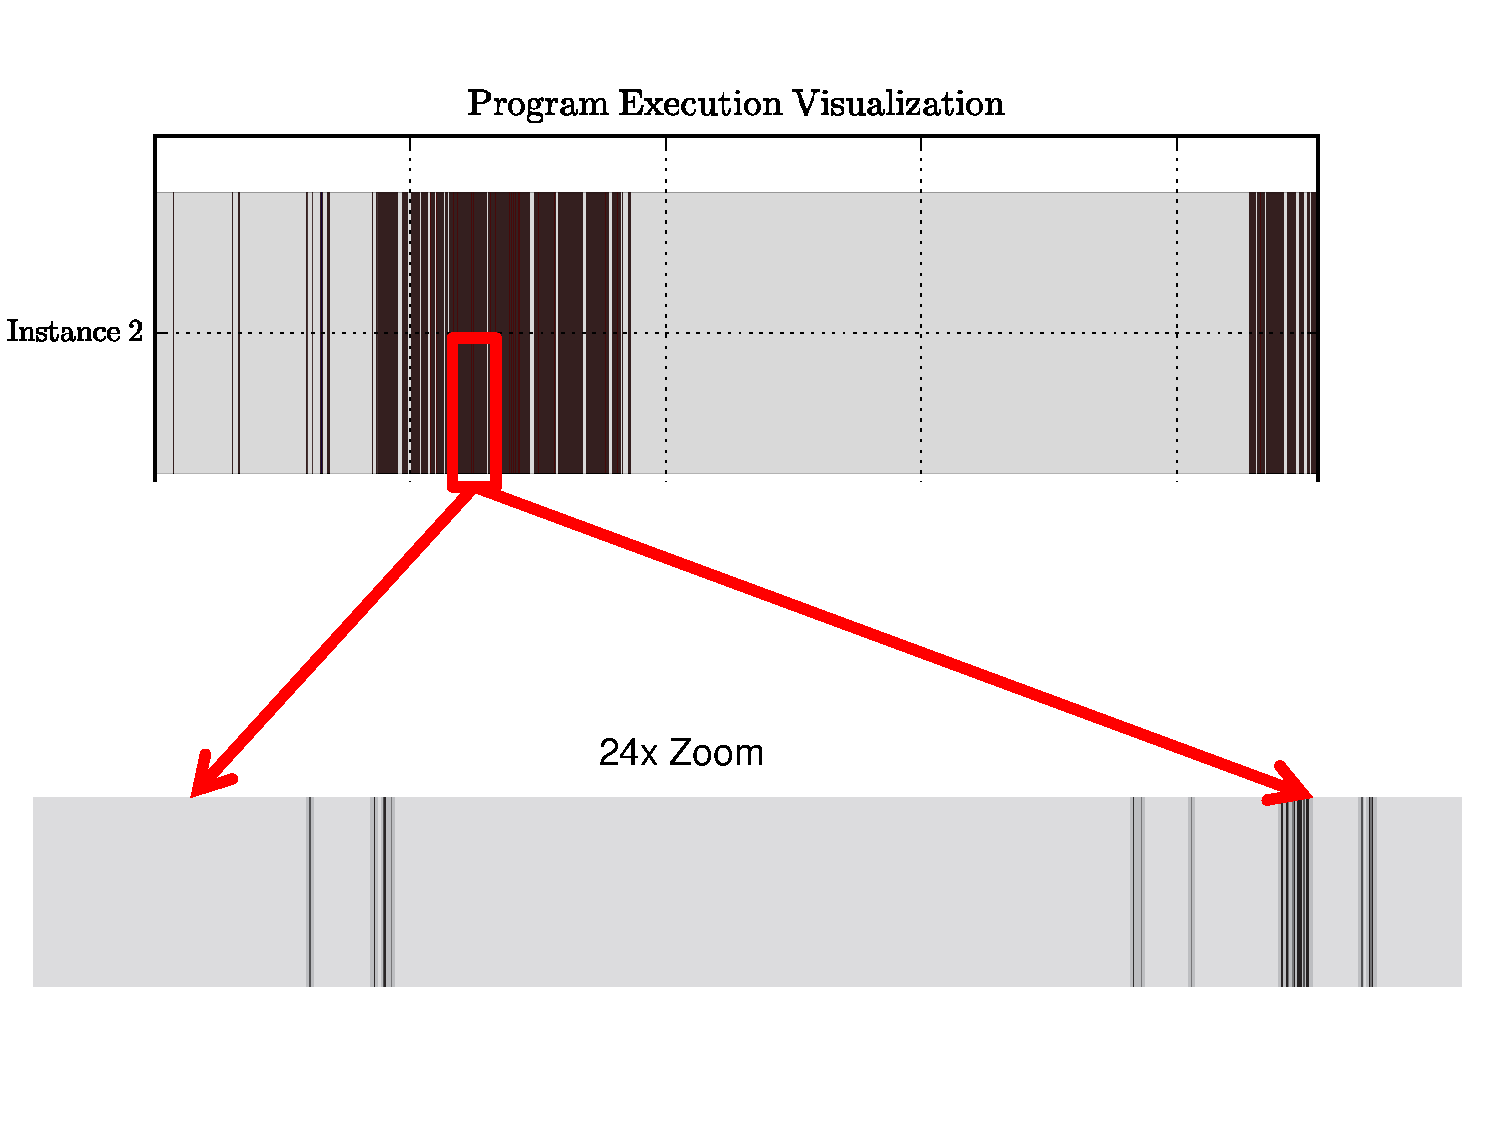
\includegraphics[trim=0cm 0cm 0cm 0cm, width=0.7\textwidth]{cronzoom-ch2.pdf}
  \caption[Understanding nature of conflicts in \texttt{cron}]%
  {Looking closely at the \texttt{cron} program execution reveals
    that conflicts occur in short bursts.}
  \label{cron:zoomtracech2}
\end{figure} 

\begin{table}
\caption{Measuring burstiness of nondeterminism in Linux services} 
\label{burst:stats}
\begin{center}
\begin{tabular}{||l|c|c|c||}\hline
  Application & Max. Consecutive Conflicts & Max. Control Flow Divergence \\
  \hline \hline
  \texttt{ntp}, 14 loop iterations & 0.03\% & 2\% 
  \\\hline
  \texttt{cron}, 30 loop iterations & 0.08\% & 0.003\% 
  \\\hline 
  \texttt{cups}, 10 loop iterations & $c$\% & $c$\% 
  \\\hline 
  \texttt{daemon A}, $i$ loop iterations & $p$\% & $ls$\% 
  \\\hline 
  \texttt{daemon B}, $i$ loop iterations & $p$\% & $ls$\% 
  \\\hline 
  \texttt{daemon C}, $i$ loop iterations & $p$\% & $ls$\% 
  \\\hline 
  \texttt{daemon D}, $i$ loop iterations & $p$\% & $ls$\% 
  \\\hline 
  \texttt{daemon E}, $i$ loop iterations & $p$\% & $ls$\% 
  \\\hline 
  \texttt{daemon F}, $i$ loop iterations & $p$\% & $ls$\% 
  \\\hline 
  \texttt{daemon G}, $i$ loop iterations & $p$\% & $ls$\% 
  \\\hline 
  \hline 
  {\bf Aggregate} & {\bf $x$}\% & {\bf $y$}\% %
  \\\hline 
\end{tabular}
\end{center}
\end{table}


\newpage \section{Summary}
This chapter presented a brief overview of the Linux boot process,
and demonstrated our methodology for both quantifying and measuring nondeterminism
in programs using dynamic instrumentation. By analyzing user-mode
instructions executed by Linux boot services and daemons, we offered
evidence that Linux services execute highly overlapping instruction
sequences across different runs. We also showed
that any conflicts or nondeterminism in such services occurs in bursts;
nondeterminism does not cause executions to permanently diverge;
divergence and convergence occur very quickly and repeatedly in our
traces.

Chapters 3 and 4 will offer insight into the sources 
of nondeterminism behind these statistics. 
Chapter 5 will look at the implications of our results for a possible
solution to the bootstorm problem.

